\documentclass[10pt,a4paper]{article}
\usepackage[utf8]{inputenc}
\usepackage{amsmath}
\usepackage{amsfonts}
\usepackage{float}
\usepackage{amssymb}
\usepackage{graphicx}
\usepackage{url}

\author{Yasar Mahomed Abbas, Franziska Pannach, \\Danielle Russell, Yuvika Singh}
\title{Report Ontologies and Knowledge Bases}

\begin{document}
\maketitle


\section{Objective and Motivation}
Folk and Fairy tales are a substantial part of oral history. They play an important role in the cultural heritage of regions, nations or cultural minorities. In European context, fairy tales have been collected and editored by the Grimm brother's in the beginning of the 19th century.\cite{Grimm1857} In the African context, the oral tradition of folk tales existed way longer. Presumably, African folk tales are therefore different than European fairy tales in terms of structure and motifs. 
This project aims to construct an ontology of African folk tales following the approach of Russian folklorist Vladimir Propp. We hope to not only collect and structure African folk tales, but also investigate how they follow Propp's formalism and how motifs and agents are verbalised.
Hence, the ontology is going to contain: 

\begin{itemize}
	\item The Proppian functions and entities encoded within. 
	\item Specific folk tale motifs according to the Aarne-Thompson-Uther Index (ATU). 
	\item The representation of the functions and motifs in selected African Folktales. 
\end{itemize}


\section{Domain}
	\subsection{Motifs Indices}
	Folk tales motifs are usually classified by two motif indices. The Aarne-Thompson-Uther index (ATU)\footnote{\url{http://www.mftd.org/}} is used to classify tales into one category. The categories are relatively wide, describing the main story line of the tale. Therefore, each tale can only have one ATU type. In contrast, the Thompson-Motif-Index (TMI) is more fine grained, describing single motifs, i.e. repeated elements, e.g. characters. The TMI motifs are organized in a hierarchical structure. A tale can be described with more than one TMI motif.\footnote{\url{https://sites.ualberta.ca/urban/Projects/English/Motif_Index.htm}}    
	\subsection{Propp Functions} 
	Russian folklorist Vladimir Propp introduced 31 invariant functions describing the morphology of the Russian magic folk tale. In his ground breaking 1928 work 'Morphology of the Folk tale', he argues that the narrative of folk tales always follows the same pattern. The narrative functions and the \textit{Dramatis Personae} (agents in the story) he introduced are strictly defined and specify recurrent units from which the tales are constructed. 
	Propp \cite{propp1968} set four axioms: 
	
	\begin{enumerate}
	
		\item Functions of characters serve as stable, constant elements in a tale, independent of how and by whom they are fulfilled. They constitute the fundamental components of a tale.
		\item The number of functions known to the fairy tale is limited.
		\item The sequence of functions is always identical.
		\item All fairy tales are of one type in regard to their structure.   
	
	\end{enumerate}
	
The high formality of this structuralism allows something as complex and highly emotional as the folk tale to be pressed in a strict pattern. Thus, they can be further used in automatically processing or when generating new tales. In Computational Linguistics, Propp's functions are used in various ways, such as for automatic markup, classification and annotation (\cite{Malec2010}), or as a foundation of an independent XML dialect (\cite{Malec2010}, \cite{Lendvai2010}). 
	His approach is still widely used not only in folk tale research but also applied to contemporary work such as the Star Wars Trilogy\footnote{http://jaced.com/2013/02/06/vladimir-propp-science-of-the-fairy-tale/}.  Proppian functions can appear in the tale as they are, with modifiers or they can be inverted, e.g. \textit{Hero leaves home} $\rightarrow$ \textit{Hero does not leave home} (explicitely).

\section{Conceptualization}
	\subsection{Existing Work} 
	Declerck et al. 2016/2017 \cite{Declerck2017} have introduced an integrated ontology that combined the ATU and the TMI motifs in a complex way. They suggested extending the ontology by including 
	
	\begin{itemize}
		\item Adding more fairy tales that fall into one of the ATU classes
		\item Adding more tales from specific collections
		\item Add Proppian functions
		
	\end{itemize}	  
	
	The aim of this project is to fulfil these three aspects. For the time being, we will concentrate on Fairy Tales anthologies from the Southern African context. Our ontology will be independent but can be easily added to the existing work once it's published by Declerck et al.\cite{Declerck2017} 
	\subsection{Definition of the Ontology}
	We describe our ontology by the following properties $<$ C,I,A,R $>$

\begin{itemize}
	
	\item $c_{i} \in C $ set of Classes: Dramatis Personae according to Propp, elements in Proppian functions, e.g. \textit{the hero}, \textit{the claim}, Proppian functions and subfunctions, classes that describe the publications of the tale (tale, anthology, editor/author)       
	\item $i_{i} \in I $ set of Instances: The representation of $c_{i}$ in the fairy tales from the anthologies such as \cite{Smith1989}, e.g. \textit{The Girl Who Lived In A Cave}, the functions appearing in those fairytales, the Dramatis Personae,  motifs according to ATU\footnote{ATU motifs in contrast to TMI motifs are not always single concepts, they can also be a description of content such as \textit{Ogre Frightened by Man} (ATU 1145-1154), nevertheless they will be classes within the scope of this project in contrast to axioms} 
	\item $a_{i} \in A$  set of Axioms: Proppian functions, e.g. \textit{Acquisition of Magical Agent}, and axioms describing the publication 
	\item $r_{i} \in R $ set of Relations: Relationships between classes that model the functions, sequential relations of functions, e.g. \textit{FollowedBy}, \textit{PrecededBy} or \textit{applies} to link the function to a tale, \textit{appearsIn} to link a Dramatis Personae to the tales, relationships linking the Dramatis Personae together, such as \textit{causesHarm}, \textit{combats} or \textit{relatedTo}
	 
\end{itemize}

We are using the ATU index for the classification of our motifs, ignoring the TMI motifs for now, since the classification of tales in TMI motifs requires a vast amount of  knowledge in literary studies. Since Declerck et al.'s ontology will cover the TMI motifs, this is not considered a drawback of our work. 

	 \subsection{Compentency Questions}
	 Our final ontology will be able to answer the following questions. 
	 
	 	\begin{enumerate}
	 		\item Which folk tales fall into a given motif class, e.g. ATU 70-99 Other Wild Animals? 
	 		\item Which Dramatis Personae appear in a given tale? 
	 	%	\item Which region do folk tales come from that fall into given motif classes? 
	 		\item Which Proppian functions appear in African folk tales? 
	 		\item How are Dramatis Personae interacting in the African folk tales, e.g. which figures use the "interdiction" relation?
	 		\item Which sequences of Proppian functions appear in the given tale?
	 		\item Which Proppian functions follow a given function predominantely, i.e. are there patterns withing the Proppian sequences? 
	 		\item Who is the editor of an anthology with folk tales from a given origin?
	 		\item How are Proppian functions verbalised, i.e. which words are used to describe events that fall into a given function class? 
	 		\item Is there a dominating interaction between certain classes of Dramatis Personae, e.g. the villain causes harm to the hero's parents?
	 	\end{enumerate}


	\subsection{Axioms}
	\label{axes}
We define some axioms for the publication and the classification of the fairy tales. 
	\small 

\begin{itemize}
		\item Each tale is published in an anthology. 
		\item Each anthology has at least one editor, a title, a publisher, and a date of publication.
		\item Each tale has a title.
		\item A tale can have an author and an origin.  
		\item Each tale has a set of Dramatis Personae. 
		\item Each person is represented by one or many verbalisations.\footnote{e.g. in Snow White 'the stepmother' and 'the evil queen' describe the same individual} 
		\item Each tale falls into one of the ATU classes. 
		\item Each ATU class has an ATU number and a description. 
		\item If a Proppian function applies for a tale, there is some verbalisation in the text. 
		\item Proppian functions follow a specific order (see below), this order is represented by a sequence. 
	%	\item Each Proppian function has a symbol. 
\end{itemize}
		
Furthermore, following Propp's approach, we derive our axioms for the possible description of the narrative as follows \cite{propp1968}: 
\begin{itemize}
	\item 	 $\alpha$ The initial situation. A text may only have a single Initial Situation function. 

\end{itemize}
\begin{enumerate}

	\item  A member of a family leaves home (the hero is introduced);
 	\item  An interdiction is addressed to the hero (’don’t go there’, ‘go to
this place’);
	\item  The interdiction is violated (villain enters the tale);
	\item  The villain makes an attempt at reconnaissance (either villain
tries to find the children/jewels etc; or intended victim questions
the villain);
 	\item  The villain gains information about the victim;
 	\item  The villain attempts to deceive the victim to take possession of
victim or victim’s belongings (trickery; villain disguised, tries to win
confidence of victim);
 	\item  Victim taken in by deception, unwittingly helping the enemy;
 	\item  Villain causes harm/injury to family member (by abduction,
theft of magical agent, spoiling crops, plunders in other forms,
causes a disappearance, expels someone, casts spell on someone,
substitutes child etc, commits murder, imprisons/detains someone,
threatens forced marriage, provides nightly torments); Alternatively,
a member of family lacks something or desires something (magical
potion etc);
 	\item  Misfortune or lack is made known, (hero is dispatched, hears
call for help etc/ alternative is that victimized hero is sent away,
freed from imprisonment);
 	\item  Seeker agrees to, or decides upon counter-action;
	\item  Hero leaves home;
 	\item  Hero is tested, interrogated, attacked etc, preparing the way
for his/her receiving magical agent or helper (donor);
 	\item  Hero reacts to actions of future donor (withstands/fails the
test, frees captive, reconciles disputants, performs service, uses
adversary’s powers against them);
 \item  Hero acquires use of a magical agent (directly transferred,
located, purchased, prepared, spontaneously appears, eaten/drunk,
help offered by other characters);
 \item  Hero is transferred, delivered or led to whereabouts of an
object of the search;
	\item  Hero and villain join in direct combat;
	\item  Hero is branded (wounded/marked, receives ring or scarf);
	 \item  Villain is defeated (killed in combat, defeated in contest, killed
while asleep, banished);
 	\item  Initial misfortune or lack is resolved (object of search
distributed, spell broken, slain person revived, captive freed);
 	\item  Hero returns;
	\item  Hero is pursued (pursuer tries to kill, eat, undermine the hero);
	\item   Hero is rescued from pursuit (obstacles delay pursuer, hero
hides or is hidden, hero transforms unrecognizably, hero saved
from attempt on his/her life);
	\item  Hero unrecognized, arrives home or in another country;
 	\item  False hero presents unfounded claims;
 	\item  Difficult task proposed to the hero (trial by ordeal, riddles, test
of strength/endurance, other tasks);
 	\item  Task is resolved;
 \item  Hero is recognized (by mark, brand, or thing given to
him/her);
 \item False hero or villain is exposed;
 \item  Hero is given a new appearance (is made whole, handsome,
new garments etc);
 \item Villain is punished;
 \item  Hero marries and ascends the throne (is rewarded/promoted).
\end{enumerate}

If a function applies for a tale, the axiom holds. Not all of the functions/axioms need to be fulfilled by every tale.
    
\subsection{Classes}
	\small 
%\begin{itemize}
Tale, Anthology, Editor, Author, Title, Publisher, Date, Fictional Person, Person, Object, ATU Class, ATU Number, Description, Proppian Function, Verbalisation, Symbol, Family Member, Hero, Villain, Victim, Seeker, Helper, Donor, Dispatcher, Princess, Princess's Father, False Hero, Magical Agent, Desired Object, Task, Reward 
%\end{itemize}


\subsection{Relations}
We define the relations based on the axioms in \ref{axes} . 

publishedIn(tale, anthology), editedBy(anthology, editor), appearsIn(fictional Person, tale), hasClass(tale, ATU), applies(tale, function), FollowedBy(function, function), PrecededBy(function, function), isInversed(function), interdicts(fictional person, hero), reconnaissance(villain, object), reconnaissance(villain, victim), gainsInformation(villain, victim), deceives(villain, victim), isDeceivedBy(victim, villain), takesPossessionFrom(villain, victim), helpTheEnemy(victim, villain), related(hero, family member), causesHarm(villain, related(hero, family member)), lacks(hero, object), testedBy(hero, donor), interrogated(hero, donor), attackedBy(hero, donor), reactsTo(hero, donor), acquires(hero, magical agent), acquiresFrom(hero, donor), ledTo(hero, desired object), combat(hero, villain), brandedBy(hero, object), defeats(hero,villain), pursuedBy(hero, fictional person), rescuedBy(hero, fictional person), proposedTo(task, hero), proposedBy(task, fictional person), resolves(hero, task), recognizedBy(hero, object), marries(hero, fictional person), isRewarded(hero, object)
\\ \\
Each of the relations describing the relationship between two fictional persons, is tied to one of the functions we described earlier. For example, if and only if the function 31. \textit{W Marriage} applies, we can use the function \textit{marries(hero, fictional person)}. That means, the relationship is tied to the appearance of the function and cannot be used in a different context, e.g. at a beginning of a tale. 
However, the application of the function \textit{W Marriage} does not guarantee that \textit{marries(hero, fictional person)} applies, e.g. when in the tale \textit{Guinea Fowl Child} the heroine is courted, the function \textit{W Wedding} still applies although there is no fictional person instance to fulfill the relationship \textit{marries}. Therefore, we cannot connect the two concepts of the class of the function and it's respective function although they belong together.   


We could formulate a relationship between the class of the Proppian function and the relation for the given example as: \\
\label{Rel}
\small
marries(A,B) $\cap$ precededBy($\bigcup\limits_{i=1}^{30}$ ProppianFunction$_{i}$)  $\cap$ $\neg$followedBy($\bigcup\limits_{i=1}^{30}$ ProppianFunction$_{i}$)
$\cap \exists $ Hero(A) $\cap \exists$ FictionalPerson(B) $\rightarrow$ ( $\exists$ W\_ Marriage $\subseteq$ applies.Tale )\footnote{The function \textit{W Wedding} is function number 31 and therefore the last function is the sequence.} \\

For the scope of this project, it is unrealistic to implement these relationsships for all 31 classes of functions and their subfunctions, especially since it is not always given that the subfunctions inherit the relationship, e.g. the \text{marries(A,B)} function applies not in case the subclass \textit{w1 Promise of marriage} applies. 

With respect to the unary relations like \textit{leavesHome(hero)}, \textit{isPunished(villain)}, we believe they are sufficiently represented by the function itself and its verbalisation, i.e. the instance of the class. The binary functions, however, allow us to model the relationships between fictional persons in a sense that would otherwise likely be lost.  

% 	leavesHome(familymember), leavesHome(hero) , misfortune(hero), decidesCounterAction(seeker), %resolvesMisfortune(object), resolvesMisfortune(fictional person), returns(hero), arrives(hero),  presentsUnfoundedClaims(falseHero), newAppearance(hero), isPunished(villain)


\normalsize
\newpage
\subsection{UML Diagram}
\begin{figure} [H]
\centering
	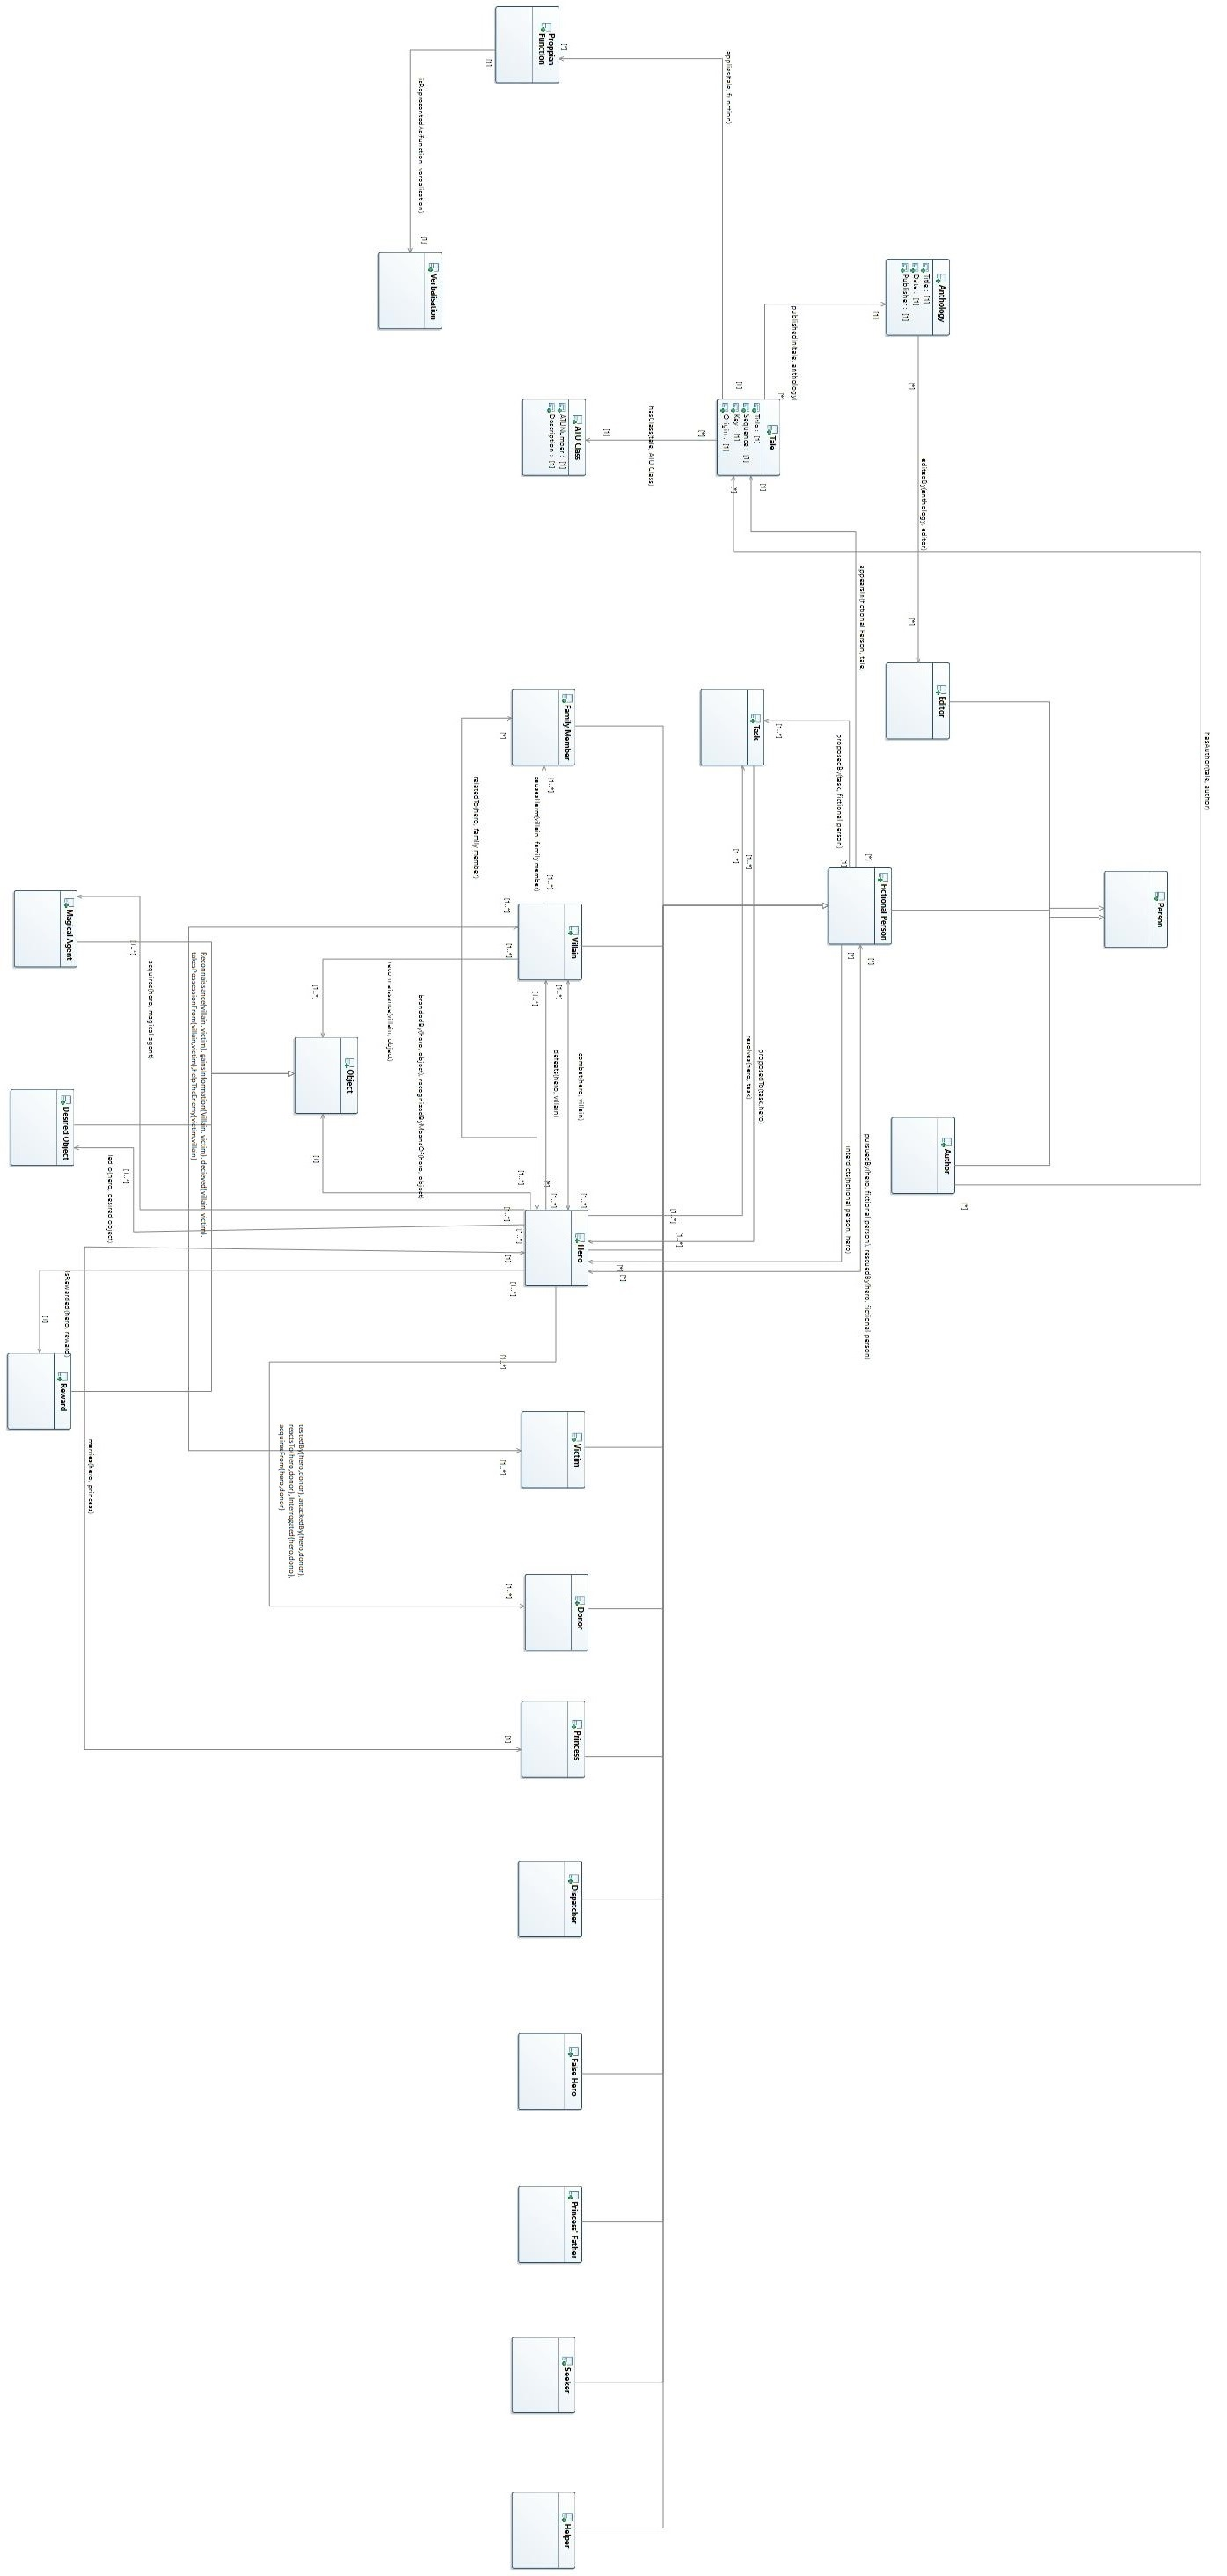
\includegraphics[scale=0.225]{UML.jpg}
\end{figure}

For the scope of this report, we refrain from putting all 31 functions and their subfunction in the UML diagram, since they are merely subfunctions of the class \textit{Proppian Function} and inherit the property \textit{Verbalisation} as well as the \textit{applies} property that connects them to the \textit{Tale} class.\footnote{In the same manner, we use Subfunction in the Description Logic representative for the 31 Proppian functions and their child functions, instead of declaring them as disjoint for each subclass.}  

\subsection{Description Logic}

The following tables describes the most important concepts of the folk tale ontology in Description Logic.
\\
\small
\begin{table}[H]
\centering

\begin{tabular}{|c|c|}
Axioms of Class Hierarchy & Important Concepts \\
\hline

FictionalPerson $\subseteq \exists $ isA.Person & FictionalPerson $\subseteq \exists$ appearsIn.Tale \\
Family Member $\subseteq \exists $ isA.FictionalPerson & Tale $\subseteq \exists$ hasClass $=$ 1 ATU$\_$Class  \\
Princess $\subseteq \exists $ isA.FictionalPerson & ProppianFunction $\subseteq \exists$ applies.Tale \\
Princess' Father $\subseteq \exists $ isA.FictionalPerson & Tale  $\subseteq \exists$ publishedIn.Anthology   \\
Hero $\subseteq \exists $ isA.FictionalPerson & Anthology $\subseteq \exists$ editedBy.Editor    \\
False Hero $\subseteq \exists $ isA.FictionalPerson & False Hero $\subseteq \neg$ Hero  \\
Victim $\subseteq \exists $ Hero $\cup$ FamilyMember $\cup$ Princess & FamilyMember $\subseteq \exists$ relatedTo.Hero \\

Dispatcher $\subseteq \exists $ isA.FictionalPerson  & Villain $\subseteq \neg$ (Victim $\cap$ Hero) \\
Villain $\subseteq \exists $ isA.FictionalPerson &  Editor  $\subseteq \neg$ FictionalPerson  \\
Donor $\subseteq \exists $ isA.FictionalPerson & Author  $\subseteq \neg$ FictionalPerson   \\
Seeker $\subseteq \exists $ isA.FictionalPerson & Reward $\subseteq \neg$ MagicalAgent  \\
Helper $\subseteq \exists $ isA.FictionalPerson & Princess $\subseteq \neg$ Princess'Father \\
Editor $\subseteq \exists $ isA.Person & \tiny SubFunction$_{i}$ $\subseteq \neg$ (ProppianFunction $\setminus$ SubFunction$_{i}$ )   \\
Author $\subseteq \exists $ isA.Person   \\
Desired Object $\subseteq \exists $ isA.Object   \\
Magical Agent $\subseteq \exists $ isA.Object  \\



\end{tabular} 
\end{table}

\section{Implementation}
In the following section, we describe the implementation of the ontology as it stands \today. 
We constructed 208 subclasses of OWL:Thing, 37 of which are disjoint. The following three pictures show a part of the classes with their respective subclasses. We followed a naming convention for the Proppian functions, trying to stay as close to the source \cite{propp1968} as possible. Propp numbered all the functions using roman letters, gave each of them a unique symbol and a short description. Therefore, our class names for the Proppian functions follow the scheme \textit{IX\_B\_Mediation}.



\begin{figure} [H]
\centering
 	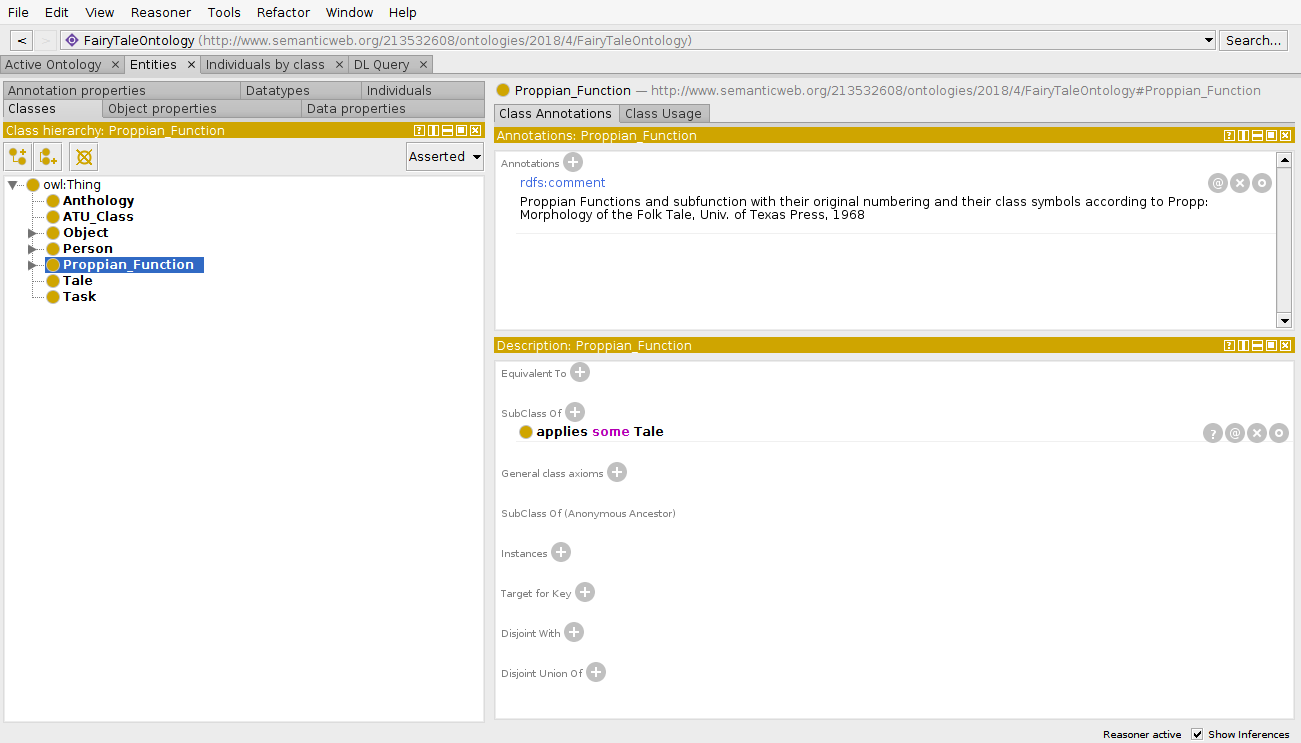
\includegraphics[scale=0.3]{Screen1.png}
 	\caption{Upper level of the subclasses}
\end{figure}

\begin{figure}[H]
\centering
 	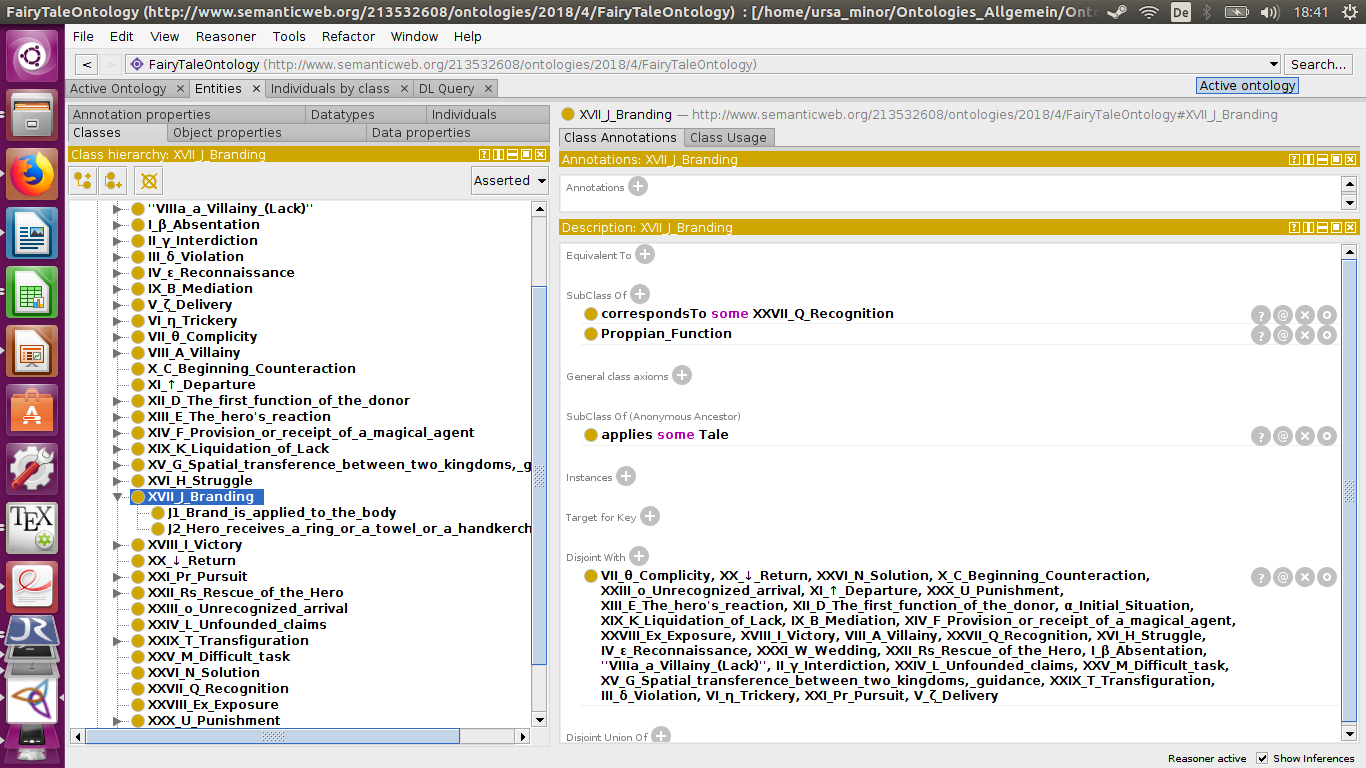
\includegraphics[scale=0.3]{Screen2.png}
 	\caption{Level of Proppian functions and their subfunctions}
\end{figure}

\begin{figure}[H]
\centering
 	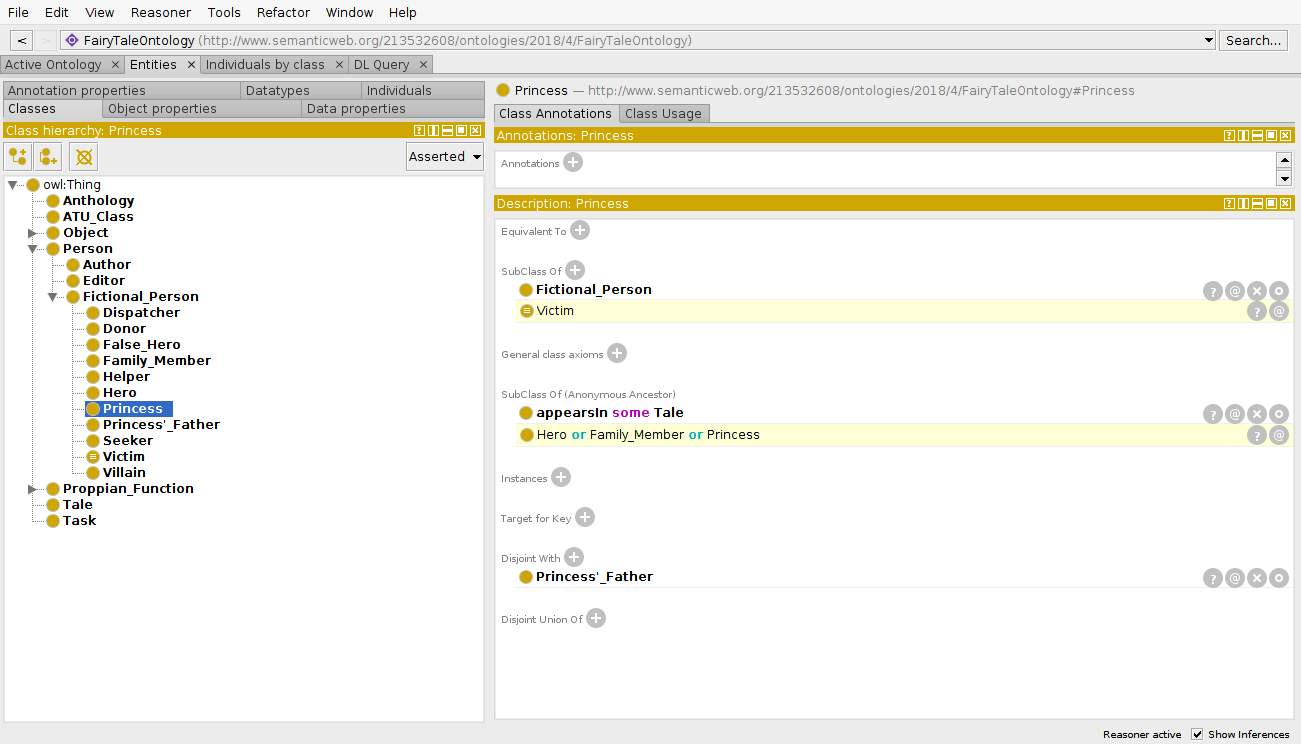
\includegraphics[scale=0.25]{Screen3.png}
 	\caption{Level of Dramatis Personae}
\end{figure}

The object properties are mainly the relations between the Dramatis Personae. They do not inherently follow a hierarchical structure. Therefore, the hierarchy of the object properties is wide but relatively flat. Where necessary, an rdf:comment describes the use of the property. 

\begin{figure}[H]
\centering
 	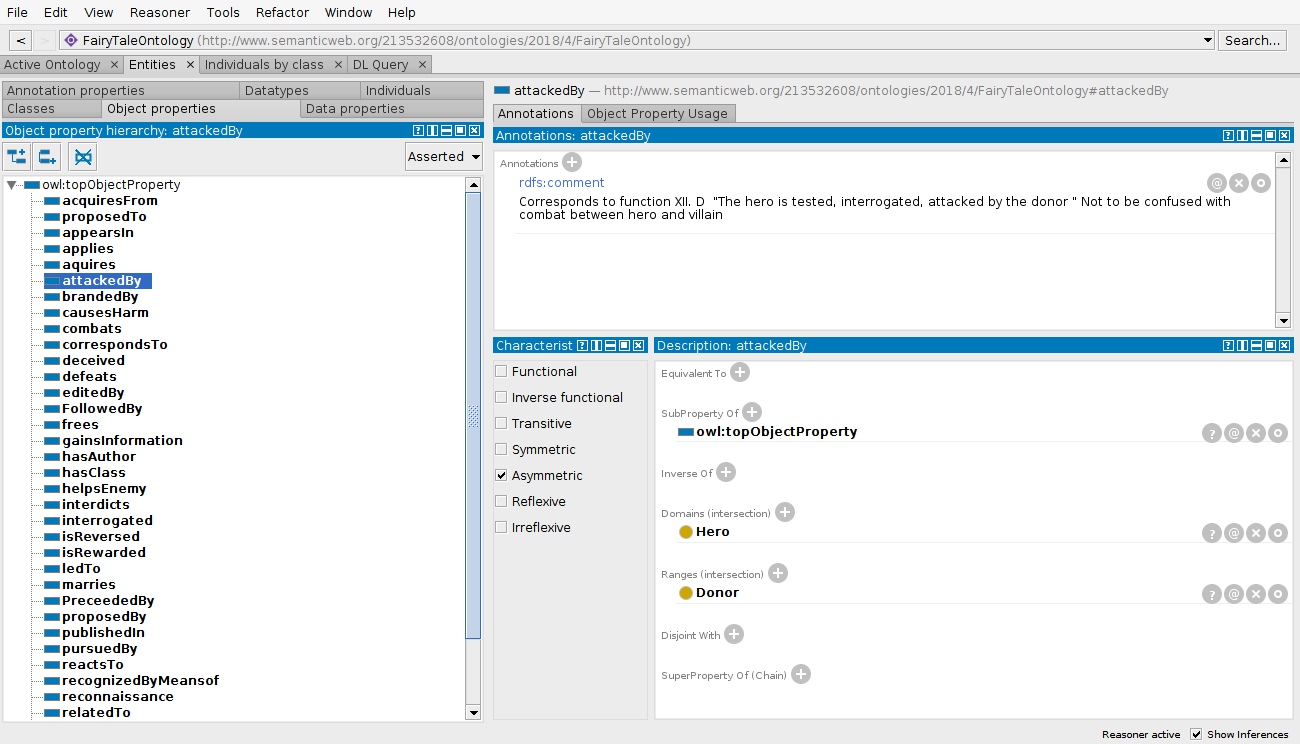
\includegraphics[scale=0.25]{Screen4.png}
 	\caption{Object Properties}
\end{figure}
\newpage

Data properties are kept relatively simple. They are used to describe the publication of the anthology, the ATU Class, the tale, or the proppian function. 
\begin{figure}[H]
\centering
 	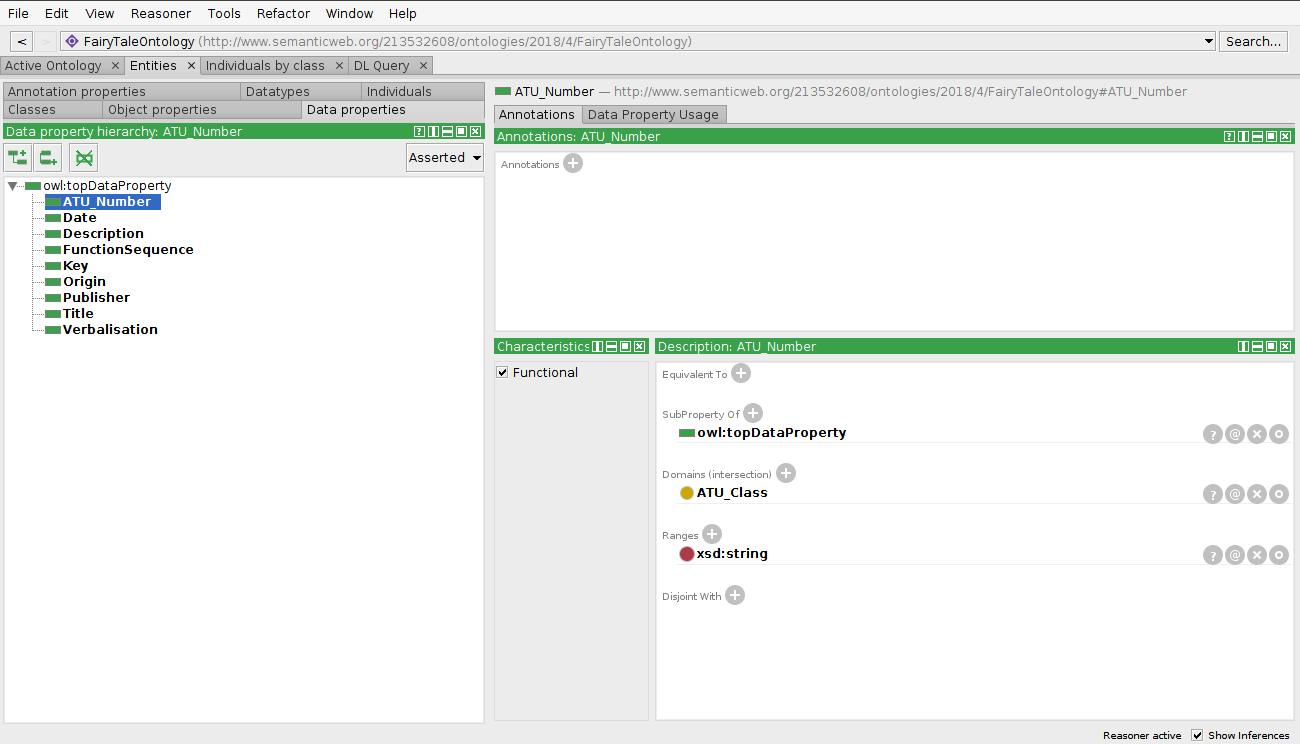
\includegraphics[scale=0.25]{Screen5.png}
 	\caption{Data Properties}
\end{figure}

We addeed the anthologies, folk tales, their ATU classes, their functions as well as the Dramatis Personae as individuals to our database. Currently, \today , we included XXXXX fairy tales, including XXXX functions and XXXX dramatis personae.
\begin{figure}[H]
\centering
 	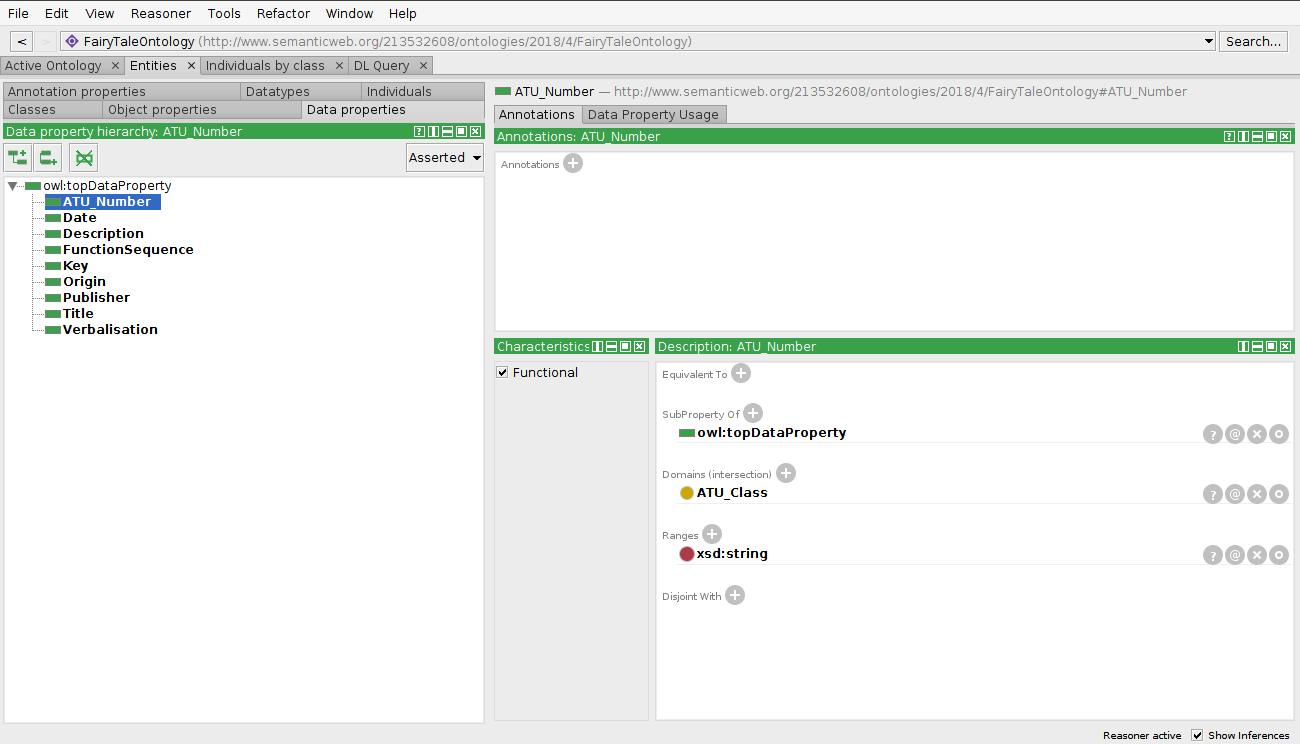
\includegraphics[scale=0.25]{Screen5.png}
 	\caption{Instances HERE INSTANCES EINFUEGEN, Wrong bild}
\end{figure}
\newpage
\subsection{Answering the Competency Questions} 

We can answer question number 1, ``Which folk tales fall into a given motif class, e.g. ATU 70-99 Other Wild Animals?" by using the DL Tab of the protege software and employing the Hermit Reasoner while querying the instances of our ontology. 
\begin{figure}[H]

\centering
 	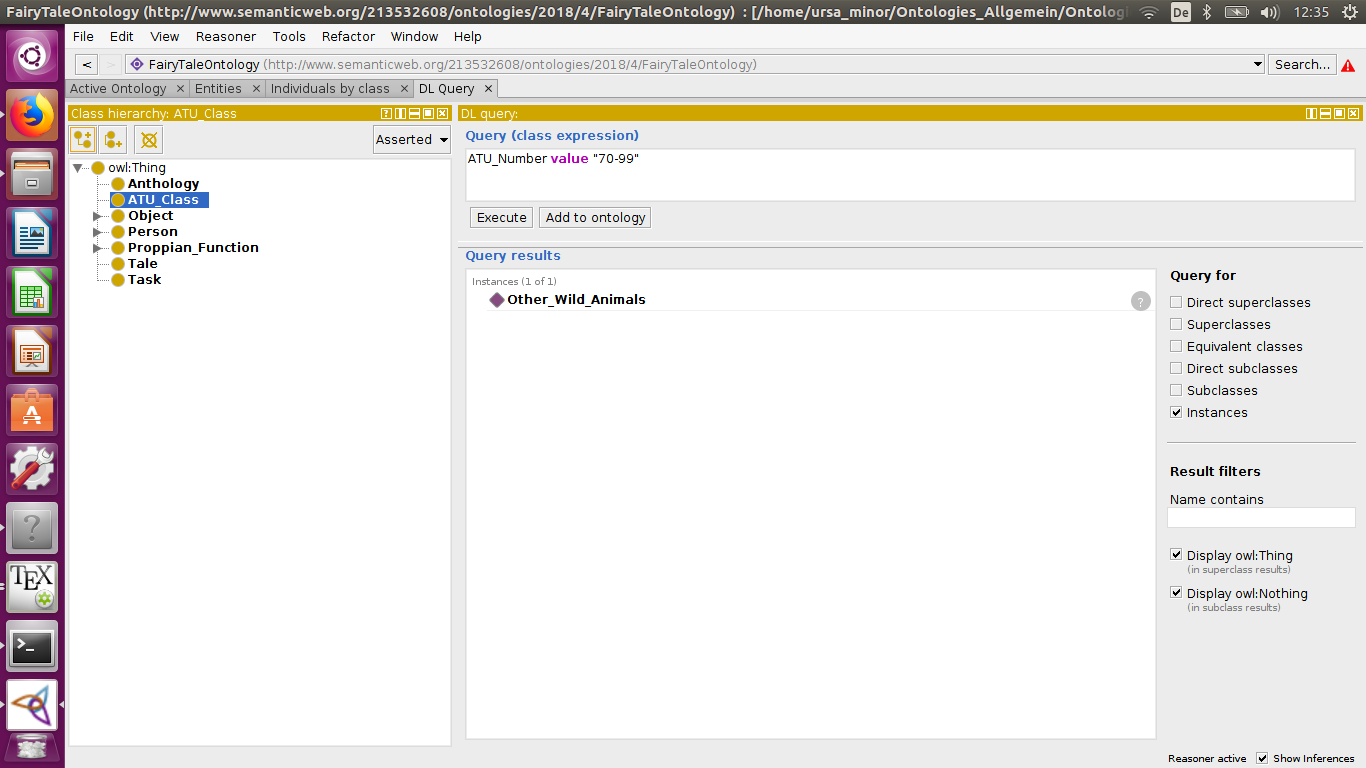
\includegraphics[scale=0.2]{Screen6.png}
 	\caption{DL Query for Competency Question 1}
\end{figure}

In the same manner, we can answer the second question ``Which Dramatis Personae appear in a given tale?". 
\begin{figure} [H]

\centering
 	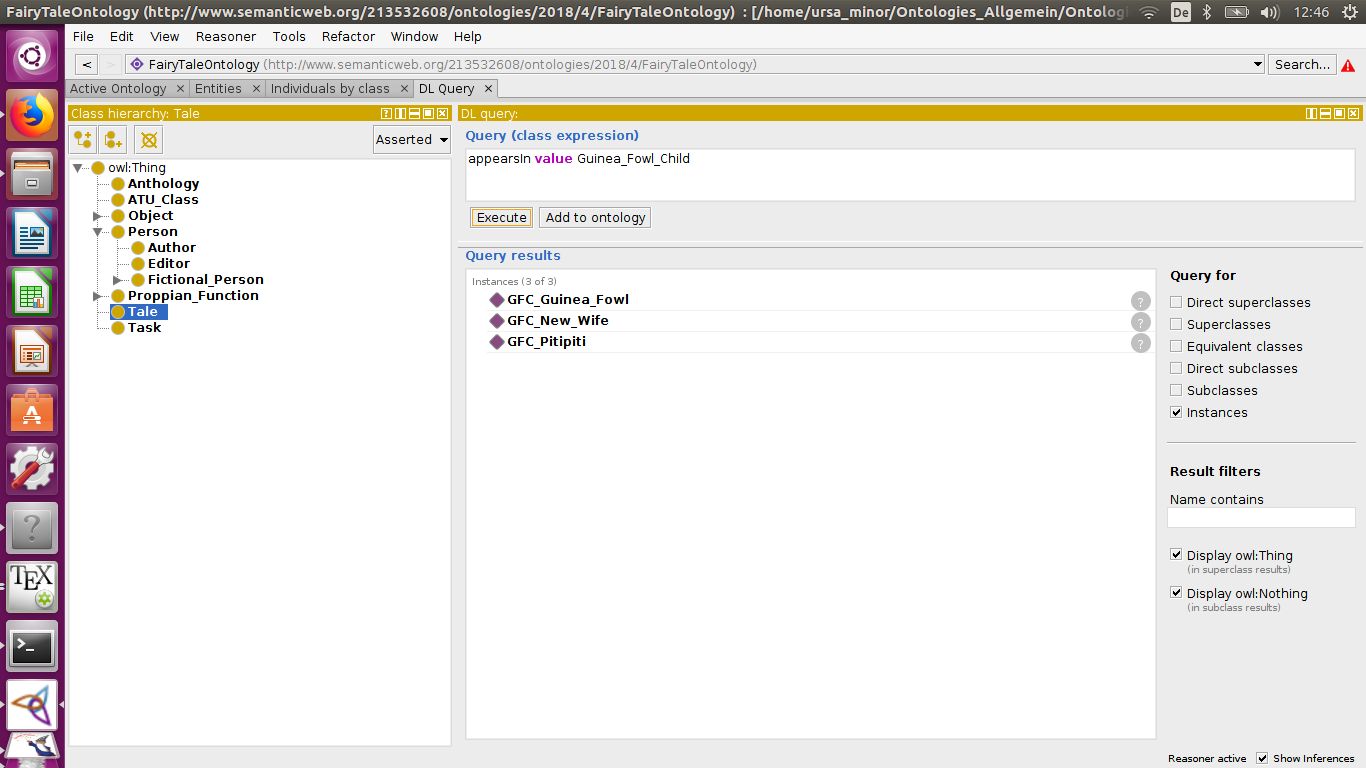
\includegraphics[scale=0.2]{Screen7.png}
 	\caption{DL Query for Competency Question 2}
\end{figure}
The answer to question 3 could be constructed as follows: 
\begin{figure} [H]
\centering
 	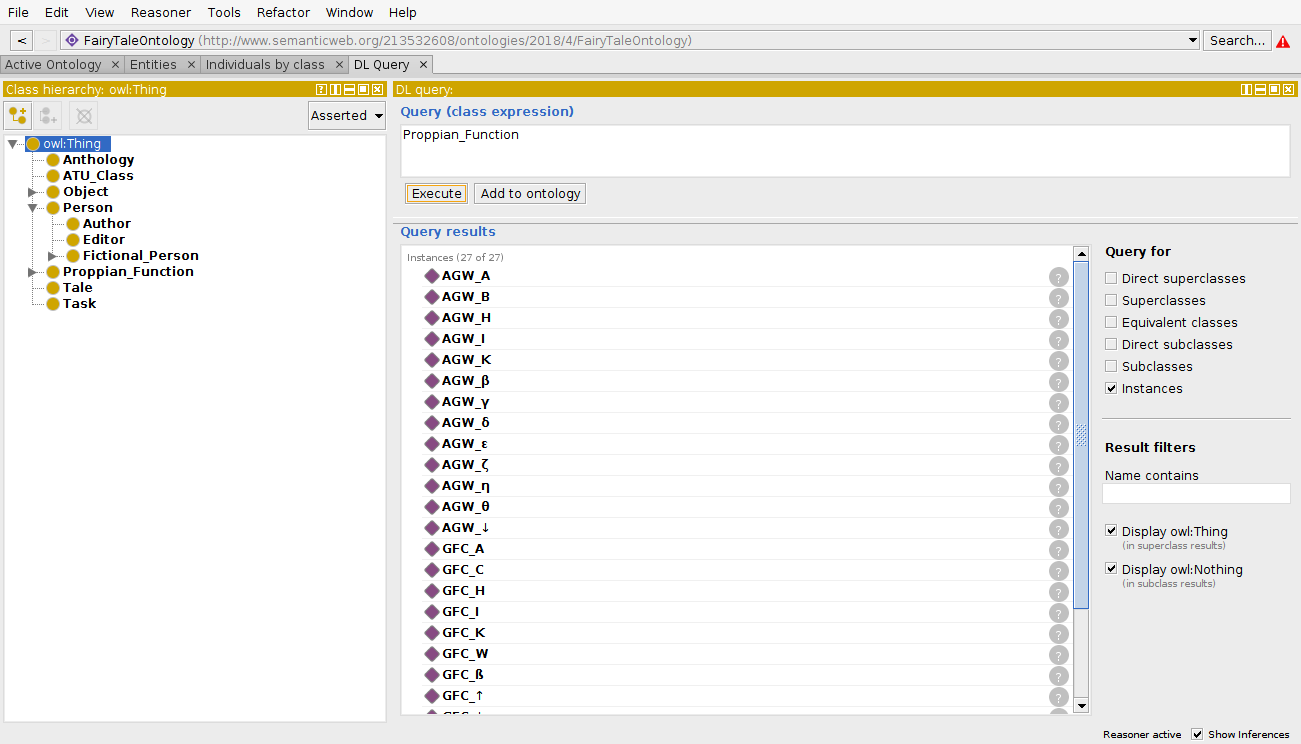
\includegraphics[scale=0.2]{Screen8.png}
 	\caption{DL Query for Competency Question 3}
\end{figure}

We can solve the question about the interaction between the Dramatis Personae, like in question 4, by querying the use of the object properties that relate to the respective function, e.g. \textit{"interdicts some Hero"}. We can query the Proppian functions of a given tale as shown in the following figure. 

\begin{figure} [H]
\centering
 	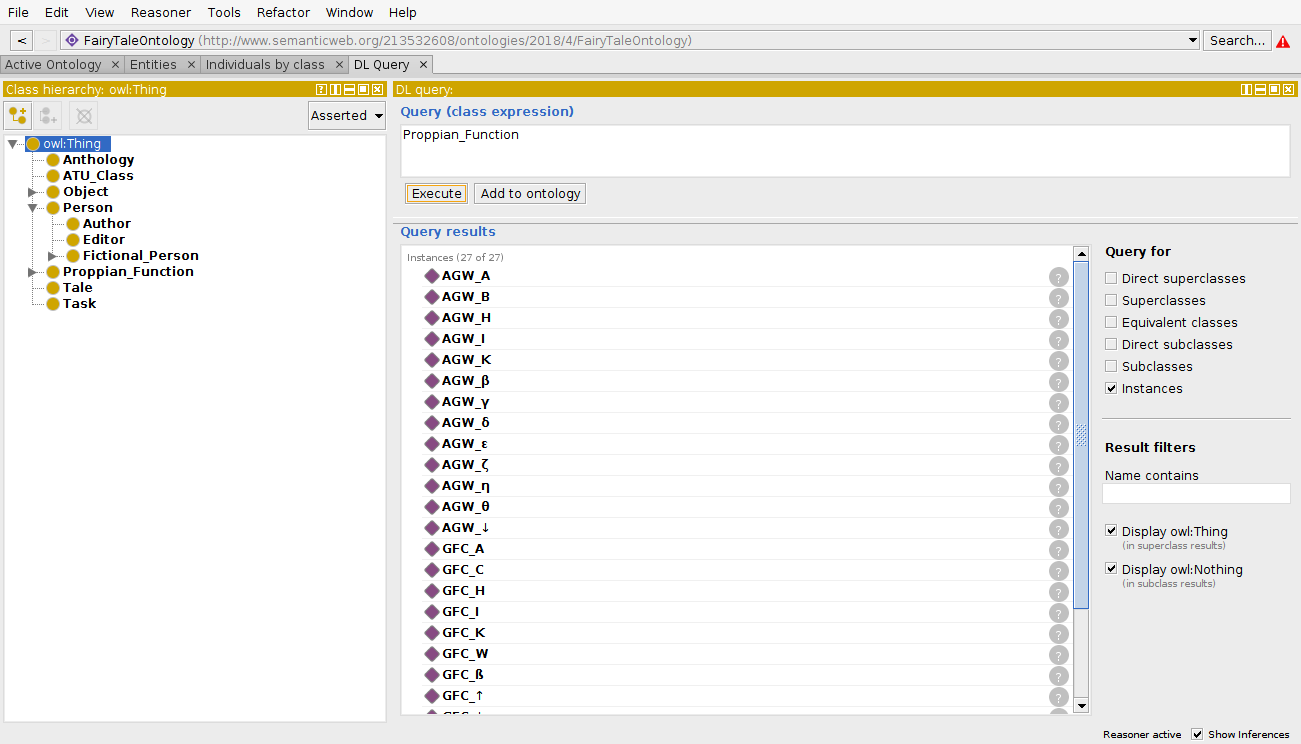
\includegraphics[scale=0.2]{Screen8.png}
 	\caption{DL Query for Competency Question 5}
\end{figure}

The more sophisticated queries such as one that would answer question number 6 can be answered using more advanced SQL-based tools. 

\newpage
\section{Conclusion and Outview}
We built a sophisticated ontology that represents the Proppian theory about the Morphology of the Folk Tale.\cite{propp1968} It also allows users to comfortably add more stories. The ontology can be alonestanding, or it can be connected to Declerck et.al.'s \cite{Declerck2017} work once their fairy tale motif ontology is published. In the long term, modelling the relationship between the functions, and the Dramatis Personae, like in the example in section \ref{Rel} could be useful. Also, adding more annotations with comments about the usage of classes of Proppian functions and their connection to the relations as described in section \ref{Rel} would certainly increase the usability of the system. Furthermore, Propp also made statements about how characters make their appearance into the course of action, a feature that could be added to the ontology in the future. 
 The more fairy tales of different origin are added, the more and complexer the deductions about the structure and verbalisation of African folk tales can be made. Certainly, these deductions can only be made with the help of scholars from folklorist or literary studies. Furthermore, it would be interesting to compare these findings about African folk tales to studies of folk tales of different origin, such as Russian, Central European or Native American tales. 
\newpage
    
\section{Bibliography}

\bibliography{Bibliography} 
\bibliographystyle{ieeetr}

\end{document}
